\documentclass[11pt,twoside,UKenglish]{scrartcl}
\usepackage{amsmath,amsfonts,amssymb}
\usepackage{textcomp,listings,fancyhdr,babel}
\usepackage[utf8]{inputenc}
\usepackage{graphicx}

\newcommand{\sintef}  {\textsc{sintef}}
\newcommand{\SINTEF}  {\textsc{SINTEF}}
\newcommand{\SAM}     {{\SINTEF} Applied Mathematics}
\newcommand{\svnrev}  {${}$Revision: 1208 ${}$}
\newcommand{\svndate} {${}$Date: 2009-01-15 13:09:30 +0100 (to, 15 jan 2009) ${}$}
\newcommand{\matlab}  {\textsc{matlab}}
\newcommand{\MATLAB}  {\textsc{MATLAB}}
\newcommand{\rstroot} {\texttt{\$RSTROOT}}
\newcommand{\matlabtm}{\matlab\texttrademark}
\newcommand{\Emacs}   {\textsc{Emacs}}

% Various definitions pertaining to MATLAB
%
\newcommand{\MATLABKeyword}[1]{\texttt{#1}}
\newcommand{\FileName}     [1]{\texttt{#1}}
\newcommand{\FunctionName} [1]{\texttt{#1}}
\newcommand{\function}        {\MATLABKeyword{function}}

\pagestyle{fancy}
\lstset{upquote}

\fancyhead{}
\fancyhead[RO,LE]{\thepage}
\fancyhead[LO,RE]{Coding Conventions}

\fancyfoot{}
\fancyfoot[LE]{\svnrev}
\fancyfoot[LO,R]{}

% Don't number any section headings.
\setcounter{secnumdepth}{-2}

\title {Coding Conventions for\\{\MATLAB} Reservoir Simulation Toolbox}
\author{{\SAM}}
\date{\svndate}

\begin{document}
\maketitle\thispagestyle{empty}
This document describes the coding conventions (coding standard)
employed in the {\MATLAB} Reservoir Simulation Toolbox (RST) developed
by {\SINTEF} Applied Mathematics (SAM).  We do not seek to codify and
enforce very detailed and rigorous standards.  However, in the interest
of achieving a consistent and readable code base, we nevertheless
highlight a few conventions which all developers should follow.  In this
document, the notation {\rstroot} refers to the absolute pathname
(directory name) of the directory in which the toolbox is physically
installed on a computer.


\section{Naming Conventions}
The toolbox is currently implemented in an imperative style using
{\function}s and scripts.  We request that unless otherwise dictated by
external concerns, user-visible toolbox {\function}s be named using
\FunctionName{lowerCamelCase}.  Specifically, function names start with a
lower-case letter and additional words start with a capital letter, for
example
\begin{verbatim}
        cartGrid
        getRelPerm
        partitionCartGrid
\end{verbatim}
The naming of non-visible functions (i.e., sub functions and nested
functions) is less rigid than for user-visible functions.  However, we
encourage developers to supply a visual cue that a given function is a
private function within a file.  In particular, we suggest that sub
functions and nested functions be named with lower-case
\FunctionName{words\_and\_underscore} such as
\begin{verbatim}
        solver
        build_system
        pick_solver
\end{verbatim}
from the function \FunctionName{solveIncompFlow} (in file
\FileName{\rstroot/pressure/solveIncompFlow.m}).


\section{Whitespace and Indentation}
Files implementing \matlab-code for the toolbox \textsl{shall} be proper
text files.  Specifically, we require that all \matlab-files (i.e.,
files whose name ends with a \texttt{.m} suffix) end with a ``line
termination character''.  Figure~\ref{fig:pref-eofnl} shows how to
configure the {\matlab} editor to automatically insert a line
termination character at the end of a file if there is none already.
Other editors (e.g., {\Emacs}) have similar configuration options.
\begin{figure}[htbp]
  \centering
  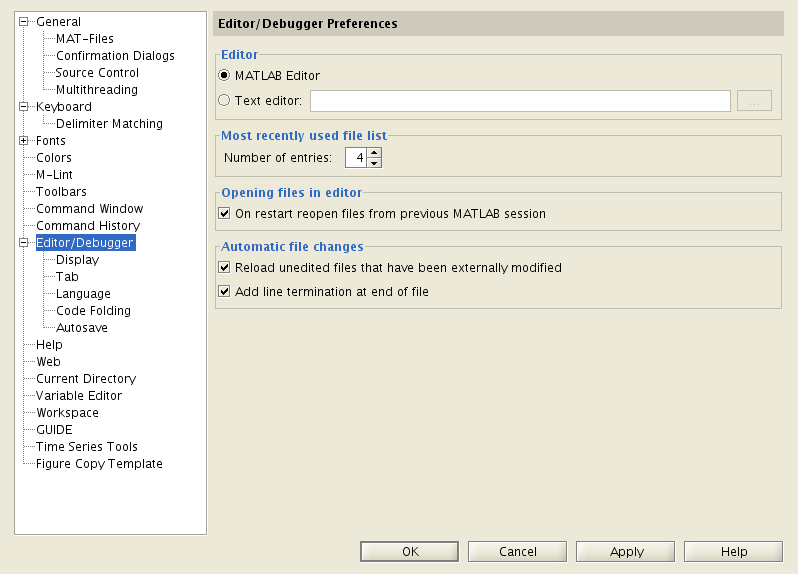
\includegraphics[width=115mm]{gfx/pref-eofnl}
  \caption{{\matlab} editor settings to have automatic insertion of a
           line termination character at end of file.}
  \label{fig:pref-eofnl}
\end{figure}
Furthermore, we request that code blocks be indented with $3$ spaces and
that all `tab's be converted to spaces.
Figure~\ref{fig:pref-tab} shows how to configure this setting in the
{\matlab} editor.
\begin{figure}[htbp]
  \centering
  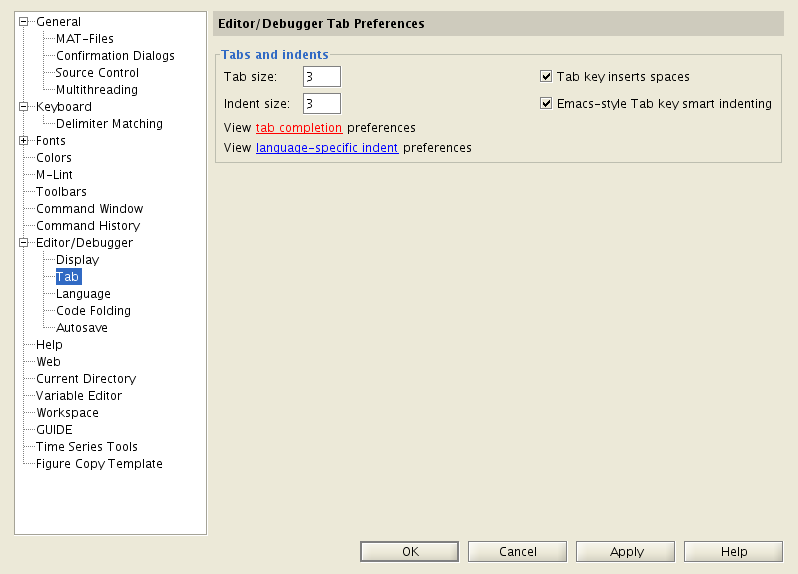
\includegraphics[width=115mm]{gfx/pref-tab}
  \caption{{\matlab} editor settings for $3$-space indents and
           conversion of tabs to spaces.}
  \label{fig:pref-tab}
\end{figure}
As a matter of formatting we ask that code lines not be overly long.
Preferably less than $80$ characters to a line.  Long expressions should
be split across several physical lines using the contination operator
`\MATLABKeyword{\ldots}' and properly indented below the existing line.
Unfortunately, the {\matlab} editor does not do proper indentation of
continued lines so this requires manual adjustments.

Finally, whitespace at end-of-line should be considered a criminal
offence whose perpetration will land you swiftly in purgatory.  The
shell function \FunctionName{eolws} defined in
Listing~\ref{shlist:fun-eolws} may be used to detect whether or not a
given file contains any EOL whitespace.  You should strive towards
{\matlab} files which produce no output other than the arrowed line
containing the file name from this function.  The function relies on GNU
\FunctionName{sed}.
\begin{lstlisting}[language=bash,float=htbp,
                   caption={\textsc{bash} function to detect end-of-line
                   whitespace.},
                   label={shlist:fun-eolws}]
          function eolws() {
              local ws='[ \t]+'
              local eol='\r?$'

              for f in "$@"; do
                  echo "============> $f"
                  sed -r -n "/$ws$eol/{=;s/$eol/$/p}" $f
              done
          }
\end{lstlisting}


\section{Guidelines for arguments in function calls}

\begin{itemize}

\item
Arguments that are also return values should be given first (not used
everywhere today.. ) proceded by structures such as G and S:

\begin{verbatim}
 G = computeGeometry(G, varargin)

 [resSol, wellSol] = solveIncompFlow(resSol, wellSol, G, S, ...
                                     fluid, varargin)

 [resSolMS, wellSolMS] = solveIncompFlowMS(resSolMS, wellSolMS, ...
                                           G, CG,  S, CS, ...
                                           fluid, varargin)

\end{verbatim}

\item
All optional arguments should be put in varargin.
\end{itemize}

\section{Documentation of functions}


Matlab-style documentation/help should be in every function file. The
documentation should be on the form displayed in the example below: 

\begin{verbatim}

function [<returnValue1>] = <functionName>(<param1>, varargin)
% <functionName> -- <Short description of function>
%
% SYNOPSIS:
%   <returnValue1> = <functionName>(<param1>)
%   <returnValue1> = <functionName>(<param1>, 'pn1', pv1, ...)
%
% DESCRIPTION:  
%  <Short description of what the function does.>
%                
% REQUIRED PARAMETERS
%  <param1>  - <description of param1> 
% 
% OPTIONAL PARAMETERS (supplied in 'key'/value pairs ('pn'/pv ...)):
%  <optParam1> - <description of param1> 
%
% RETURNS:
%  <returnValue1>   - <description of returnValue1>
%
% EXAMPLE:
%   <Display a short example of use of the function or refer to a file
%   containing a more detailed example.> 
%
% (REMARKS:)
%   <list any additional requirements/remarks>
%
% SEE ALSO:
%   <list of relevant functions>
%                                     
% (TODO:)
%   <list of needed functionality>
\end{verbatim}
The arguments enclosed in parentheses are only included when needed. 

\end{document}


%%% Local Variables:
%%% mode:LaTeX
%%% TeX-master:t
%%% fill-column:72
%%% End:

% vim: si et tw=72 sw=2 fo=tcroql com=b\:\%
